%%%%%%%%%%%%%%%%%%%%%%%%%%%%%%%%%%%%%%%%%
% Journal Article
% LaTeX Template
% Version 1.4 (15/5/16)
%
% This template has been downloaded from:
% http://www.LaTeXTemplates.com
%
% Original author:
% Frits Wenneker (http://www.howtotex.com) with extensive modifications by
% Vel (vel@LaTeXTemplates.com)


%----------------------------------------------------------------------------------------
%	PACKAGES AND OTHER DOCUMENT CONFIGURATIONS
%----------------------------------------------------------------------------------------

\documentclass[twoside,twocolumn]{article}

\usepackage{color,soul}
\usepackage{graphicx}
\graphicspath{{./figures/}}


% Colors
\definecolor{blu}{rgb}{0,0,1}
\def\blu#1{{\color{blu}#1}}
\definecolor{gre}{rgb}{0,.5,0}
\def\gre#1{{\color{gre}#1}}
\definecolor{red}{rgb}{1,0,0}
\def\red#1{{\color{red}#1}}
\definecolor{lblu}{RGB}{10,213,216}
\def\lblu#1{{\color{lblu}#1}}

\def\image#1#2{{\includegraphics[scale=#2]{#1}}}
\def\html#1{{\textless#1\textgreater ... \textless/#1\textgreater}}

%Template
%\definecolor{x}{rgb}{0,0,0}
%\def\x#1{\color{x}#1}
\setul{0.5ex}{0.3ex}
\setulcolor{red}
% LaTeX
\def\items#1{\begin{itemize}#1\end{itemize}}
\def\enum#1{\begin{enumerate}#1\end{enumerate}}

\usepackage{blindtext} % Package to generate dummy text throughout this template 

\usepackage[sc]{mathpazo} % Use the Palatino font
\usepackage[T1]{fontenc} % Use 8-bit encoding that has 256 glyphs
\linespread{1.05} % Line spacing - Palatino needs more space between lines
\usepackage{microtype} % Slightly tweak font spacing for aesthetics

\usepackage[english]{babel} % Language hyphenation and typographical rules

\usepackage[hmarginratio=1:1,top=32mm,columnsep=20pt]{geometry} % Document margins
\usepackage[hang, small,labelfont=bf,up,textfont=it,up]{caption} % Custom captions under/above floats in tables or figures
\usepackage{booktabs} % Horizontal rules in tables

\usepackage{lettrine} % The lettrine is the first enlarged letter at the beginning of the text

\usepackage{enumitem} % Customized lists
\setlist[itemize]{noitemsep} % Make itemize lists more compact

\usepackage{abstract} % Allows abstract customization
\renewcommand{\abstractnamefont}{\normalfont\bfseries} % Set the "Abstract" text to bold
\renewcommand{\abstracttextfont}{\normalfont\small\itshape} % Set the abstract itself to small italic text

\usepackage{titlesec} % Allows customization of titles
\renewcommand\thesection{\Roman{section}} % Roman numerals for the sections
\renewcommand\thesubsection{\roman{subsection}} % roman numerals for subsections
\titleformat{\section}[block]{\large\scshape\centering}{\thesection.}{1em}{} % Change the look of the section titles
\titleformat{\subsection}[block]{\large}{\thesubsection.}{1em}{} % Change the look of the section titles

\usepackage{fancyhdr} % Headers and footers
\pagestyle{fancy} % All pages have headers and footers
\fancyhead{} % Blank out the default header
\fancyfoot{} % Blank out the default footer
\fancyhead[C]{COGS 402 Project $\bullet$ Winter Term 2, 2019} % Custom header text
\fancyfoot[RO,LE]{\thepage} % Custom footer text

\usepackage{titling} % Customizing the title section

\usepackage{hyperref} % For hyperlinks in the PDF

%----------------------------------------------------------------------------------------
%	TITLE SECTION
%----------------------------------------------------------------------------------------

\setlength{\droptitle}{-4\baselineskip} % Move the title up

\pretitle{\begin{center}\Huge\bfseries} % Article title formatting
\posttitle{\end{center}} % Article title closing formatting
\title{Convergent validity analysis of developing a gambling cognitions scale} % Article

%Alternative title: Concurrent study of developing a scale to measure cognitive distortions

\author{%
  \textsc{Muhammad Ali} \\[1ex] % Your name
\normalsize Student Number: 39738142 \\
\normalsize COGS 402 \\ % Your institution
\normalsize \href{mailto:muhammad.ali.72.27@gmail.com.com}{muhammad.ali.72.27@gmail.com} % Your email address
%\and % Uncomment if 2 authors are required, duplicate these 4 lines if more
%\textsc{Jane Smith}\thanks{Corresponding author} \\[1ex] % Second author's name
%\normalsize University of Utah \\ % Second author's institution
%\normalsize \href{mailto:jane@smith.com}{jane@smith.com} % Second author's email address
}
\date{\today} % Leave empty to omit a date
\renewcommand{\maketitlehookd}{%
\begin{abstract}
  \noindent This study investigates the development and measuring of gambling related cognitions by performing a convergent validity analysis between existing scales such as the Belief in Good Luck scale and the Gambling related Cognitions Scale. The purpose was to elicit a gambling experience that would be reflected as scores on the state scale which is the scale being developed. These scores and the questions that elicited them were filtered through exploratory factor analysis and then compared with existing scales to measure their convergent validity. It was hypothesized that the scores on the state scale will be highly related to similar subscales on the Belief in Good luck scale and the Gambling Related Cognitions scale.
\end{abstract}
}

%----------------------------------------------------------------------------------------

\begin{document}

% Print the title
\maketitle

%----------------------------------------------------------------------------------------
%	ARTICLE CONTENTS
%----------------------------------------------------------------------------------------

\section{Introduction}

\lettrine[nindent=0em,lines=3]{T}he aim of this article is to uncover the way a gambling experience can influence the degree of belief in gambling fallacies. A majority of BC residents gamble such that it accounts for 3 in 4 adult B.C. residents \cite{bclc}. Additionally, these players have higher than average household incomes with more than three quarters of players having post-secondary or higher education \cite{bclc}. This is important because if you consider that these players are inclined to play within a year, a question that might naturally arise is how many of these players hold beliefs in gambling fallacies. Even though there does not exist a causal relationship between the conviction of erroneous beliefs and problematic gambling, there are strong relationships reported in studies to suggest otherwise \cite{Ladouceur:2004, raylu:2004, darke:1997}. With these erroneous beliefs, there exists other health implications such as substance use disorders that accompany problematic gamblers \cite{rush:2008}. If you consider the probability of about 75\% of B.C. residents gambling within the past year, it is reasonable to suggest that a subset of these people are more likely than others to develop problematic gambling habits and possible substance use disorders \cite{bclc}. In order to increase awareness in the identification of these erroneous beliefs, this study attempts to develop a scale to accurately identify the beliefs held as a result of slot machine gameplay. The scale, which is called the state scale in this study, would aid in clinical diagnosis such that it would be able to provide a clear measure of determining whether someone is likely to engage in problematic gambling; although this scale does not attempt to provide a diagnostic tool, it can aid in clarifying misconceptions and in research related to problematic gambling.

I first need to introduce the difference between cognitive distortions and gambling fallacies. Cognitive distortions refer to erroneous beliefs held, for the purpose of this study, by problematic gamblers. These distortions are not a result of pathological gambling but rather comprise a set of beliefs commonly found in non-gamblers alike. These beliefs are more apparent in people that are diagnosed to be problematic gamblers \cite{Ladouceur:2004}. The classification of these erroneous beliefs are referred to as \emph{gambling fallacies}. These fallacies arise in individuals in the form of the belief that chance events can be controlled, that there is an insensitivity to sample size, believing opposite results are more likely in random events etc.\cite{Leonard:2015}.

The breadth of the gambling fallacies addressed by the state scale are:
\begin{description}
\item[\textbf{The Hot hand fallacy:}] a winning streak of symbols on the slot machine are more likely to appear than symbols that do not produce wins \cite{Leonard:2015}. For example, if a person received consecutive wins, he/she will expect another win to be more probable. 
\item[\textbf{Belief in luck: }] randomly determined outcomes of the slot machine favour certain things over others in a way that is dispositional \cite{Leonard:2015}. For example, having a "lucky" day whenever placing bets in a game of chance increases the odds of winning.
\item[\textbf{Illusion of control:}] It is the tendency to believe that actions influence wins \cite{Leonard:2015}. For example, a person would think that touching the screen at a certain location would result in a win.
\item[\textbf{The Gambler's fallacy:}] It is expecting the opposite outcome of an event to be more likely such that standard deviation in random events are corrected so that wins "even out" \cite{Leonard:2015}.
\item[\textbf{Anthropomorphic:}] This is assigning distinct human characteristics to nonhuman objects \cite{wyatz:2010}. For example, if after receiving no wins through a prolonged period of time, you might expect that the machine was overtly biased. 
\item[\textbf{Supernatural:}] This is the belief that the result of wins was due to a situation out of the persons control but a thing that still exerts a \emph{secondary} illusion of control \cite{ejova:2015}. For example, someone might consider a mystical force or even religion in order to explain their winnings.
\end{description}

Although not typically considered a gambling fallacy, anthropomorphism in included because some literature has suggested that these beliefs suggest a source of influence on erroneous beliefs \cite{wyatz:2010}. Since gambling fallacies are a result of higher than normal amount of erroneous beliefs, the social influence anthropomorphism asserts might attribute to an increase in these beliefs \cite{wyatz:2010}. Since there are no clear distinctions between cognitive distortions labelled as gambling fallacies it is helpful to include the additional beliefs \cite{Leonard:2015}

Now that I have listed the set of gambling fallacies and their explanations, it is important to review the problems associated with this field of literature; the field lacks consensus as to what specific behaviour constitutes gambling fallacies and what instruments best assess them \cite{Leonard:2015}. The first issue addresses the measurement of cognition which I admit is difficult to achieve simply by asking for self-reports. However, previous scales have been developed that admit high internal validity and reliability across studies that address specific gambling fallacies among a general set of cognitive distortions; this is encouraging when considering that reliable scales were also developed via self-reports\cite{Leonard:2015, Ladouceur:2004,raylu:2004, darke:1997, wyatz:2010}. Each of these scales admit a high degree of reliability and so being able to validate against them would provide novel information about the effectiveness of the state scale; the degree of internal validity (i.e. Cronbach's $\alpha$) can be found in table 1. The only drawback of these scales is that they only measure specific gambling related cognitions, like the Belief in Good Luck Scale (BIGLS) \cite{Leonard:2015}. The exception is the Gambling Related Cognitions Scale (GRCS) which is used frequently in measuring gambling related cognitions \cite{gabriel}. However, it lacks some commonly associated cognitive distortions associated with problematic gambling like the hot hand fallacy or gambler's fallacy \cite{raylu:2004}. The fact that the GRCS has sub scales that measure a limited scope of beliefs lends to the idea that one could possibly develop a scale that measures the breadth of gambling fallacies while also taking into account that there are no clear distinctions in gambling fallacies and erroneous beliefs. Secondly, the measures of these gambling fallacies is less difficult when considering the reliability that the GRCS and BIGLS offer \cite{Leonard:2015}. This would suggest that being able to correlate the previously validated scales with the state scale allows for a clear measure of those gambling fallacies that are not mentioned in the GRCS or BIGLS; the questions that test for subscales in existing scales should be clear and those beliefs that are unique to the state scale could provide novel information.

Additionally, there are other studies that provide evidence for the question of whether asking participants to answer questions on a survey would truthfully reveal the gambling fallacies. This area of research is addressed by Sevigny and Ladouceur who conducted a study on "The double switching concept" in 2003; they found that before and after a gambling experience, participants changed the degree of their beliefs. More specifically, they found that participants would shift from a rational perception of gambling (switch on) to a behavioural manifestation of erroneous beliefs (switch off) and then go back to a rational perception (switch on) \cite{sevigny:2003}. This would suggest that after a gambling experience, participants elicit a greater degree of erroneous belief and even verbalize thoughts accordingly \cite{sevigny:2003}. This particular research is interesting and is even introduced in a study around pathological gambling; the verbalization is particularly important, not only for this study, but for the study on pathological and non-pathological gamblers \cite{Ladouceur:2004}; for this study, it suggests that after playing with a slot machine, participants should elicit changes in their beliefs around gambling fallacies.The study focused around pathological gamblers that elicited high degrees of erroneous beliefs found that gamblers verbalized significantly more "gambling related perceptions and were more convinced in the truth of their perceptions than non-problem gamblers" \cite{Ladouceur:2004}. These verbalizations included references to things related to gambling fallacies like cause and effect, superstition, inappropriate attribution, or personal control \cite{Ladouceur:2004}. At the end of this study and others on gambling fallacies, it is suggested that not many longitudinal studies exist measuring the attribution of erroneous beliefs to problematic gambling \cite{Leonard:2015, Ladouceur:2004, raylu:2004}. However, this is partly addressed by a twin study that controls for confounding genetic and environmental influences on pathological gambling and cognitive distortions \cite{xian:2008}. The twin study found high internal reliability reported by the Cronbach alpha coefficient while also reporting that sociodemographic characteristics (i.e. marital status, education, employment, annual income etc.) were not related to the degree of cognitive distortions \cite{xian:2008, cronbach}. This is evidenced by the fact that people who have post secondary and higher education also partake in gambling related activities \cite{bclc}. It is useful for this study since the participants are acquired from a university population in which the reported degree of gambling is not high; it suggests that the sociodemographic characteristics like education do not assert a strong influence and what does is the degree of conviction in erroneous beliefs.


The purpose of this research is to develop a scale but more specifically to test how values gained during experimentation reveal latent factors that are the result of a gambling experience. Rather than test for independent cognitive distortions as reported scales such as the Belief in Good Luck scale (BIGLS) attempt to do, the aim was to develop a scale to measure gambling-related cognitive distortions during a gambling session \cite{darke:1997, Leonard:2015}. Then, to validate the identified latent factors to existing scales. The assumption was that, for people who score highly on one measure such as luck on the state scale would also score similarly in the already existing scales such as the BIGLS or GRCS; this allows for a relationship to measure the discrepancy on the values reported in the state scale and other scales. In summary, the aim was to develop a questionaire that would test the cognitive distortions as outlined through previously identified research by validating the results against existing and reliable scales to see if a subset of factor measures can accurately predict individual gambling fallacies in slot machine gameplay. \cite{Leonard:2015}

%------------------------------------------------

\section{Methods}

\subsection{Participants}
The participants were gathered from the human subject pool (HSP) provided by the department of psychology with 101  of these participants filling out the scale being developed. Participants needed to have demonstrated a proficiency in English, normal or corrected-to-normal vision, not have experienced gambling either now or in the past, and not be taking medications to treat any mental health problems. Participant scores were also used form the Pilot study in which 87 participants were recruited from the HSP.

\subsection{Procedure}
The participants of the study were instructed prior to the gambling session that the study was "measuring state beliefs about gambling" which was left open-ended so that their scores would not be affected by their perception of what is expected of them. After reading over the consent form provided by the Center for Gambling Research lab at the University of British Columbia, the participants filled out the Canadian Problem Gambling Index (CGPI). The CGPI is used to assess the risk for problematic gambling\cite{wynne:2003}. However, the GRCS and the BIGLS scale both used the South Oaks Gambling Scale (SOGS) to assess problematic gambling; as a result of gathering participants from the HSP, there were no counts of high CGPI scores\cite{darke:1997, raylu:2004}. This would indicate that an extensive scale such as SOGS is not needed to assess problematic gambling and the CGPI scale is sufficient. The participants were then further instructed to complete the GRCS and BIGLS questionnaires. Afterwards, they were directed to play a slot machine session in which they were given \$40 to place bets with; the participants would be rewarded with a sixth of the total amount rounded to the nearest quarter. Additionally, the participants were told that they should place bets keeping in mind that they have a real stake in the outcome of the game. Afterwards, they were instructed to fill out the State questionaire with the gambling experience in mind. At the end of their survey, they were debriefed of the purpose of the study and related literature.

The scores that were gathered from the GRCS, BIGLS, and State survey were collected as entries of a spreadsheet which was then turned into matrices for statistical manipulation. The State survey itself was a 7-point likert scale that consisted of questions probing the previously listed gambling fallacies. It should be noted that there was no intention of testing overlapping constructs; for example, having a question that measured both the  illusion of control and the gambler's fallacy was left out.
\subsection{Exploratory Factor Analysis (EFA)}
It should be noted that the EFA procedure was used primarily to find differences between questions and how well they identified latent constructs. This means that questions that identified poorly with more than one latent construct were subject to removal; for example, if a question gave a low relationship value between luck and illusion of control then it would be removed. The statistical analysis was done in python with the standard packages for data analysis such as Pandas (Data collection), Numpy (Data manipulation), FactorAnalyzer (EFA analysis), and Matplotlib (for plotting statistics) \cite{factoranalyzer}.

The scores that were gathered were represented as matrices in which the rows indicated the score each participant gave and columns indicated the questions that were asked. According to standard EFA procedures, the correlation matrix was gathered for the State scale so that potential questions that had numerous values under 0.3 or only a small amount greater than 0.3 were removed \cite{efa}. Additionally, the correlation matrix is a symmetric matrix where the rows and columns are the list of questions; this is done to see how the scores of individual questions related to each other \cite{efa}.

After the correlation matrix was analyzed to potentially include items for removal, the determinant was calculated so that the suitability of the data could be assessed for performing EFA \cite{efa}. The nature of EFA of this study is such that questions would be removed based on how well they identified latent constructs so for each removal of a question the entire procedure would have to be repeated. This iterative procedure is due to the fact that removal of a question in a survey could significantly alter the constructs that are measured; it affects the correlational relationship between each individual question. Afterwards, the determinant was calculated in order to determine the suitability of the data; if the determinant of the matrix was <0.00001 then it indicated the values retained were suitable for EFA analysis. In addition to identifying the determinant, the Kaiser-Myer-Olkin (KMO) value was also calculated to check the matrix for suitability as well \cite{efa}. The difference between a determinant and the KMO value is such that the KMO value checks whether the sample size was adequate for EFA \cite{efa}. With respect to the KMO value, there is an associated \emph{anti-image matrix} which is a matrix of the KMO values for individual questions. This anti-image matrix was also used to eliminate questions that had low KMO values indicating that the sample size was not identifying clear distinctions between participant scores \cite{efa}.

However, when the EFA was performed using FactorAnalyzer the "quartimin" rotation was used \cite{factoranalyzer}. The reason for this rotation is because it is difficult to measure gambling related cognitions so it is reasonable to expect that multiple questions could be measuring some constructs more closely than others (i.e. the difference between the questions isn't orthogonal)\cite{efa}. This would allow the EFA procedure to better identify the relationship between questions such that it is not constrained to looking for one construct \emph{or} the other but rather fit according to the shape of the data \cite{efa}. The latent factors were identified using Eigenvalues for each questions; these are values that are typically "solutions" to a matrix and provide unique discrete numbers \cite{lay}. The cutoff used to determine how many latent factors there were was done through eigenvalues "greater than one" \cite{efa}. Put simply, these values determine how many latent factors are being measured with each eigenvalue identifying questions that predict a latent construct. If for example, I found three eigenvalues greater than 1, then I could reasonably conclude the questionaire is measuring three gambling fallacies \cite{efa, lay}.

Lastly, the factor loadings were calculated \cite{factoranalyzer}. These are the most important values because they determine which questions map on to their particular latent construct \cite{efa}. It is typical convention  to remove values less than 0.3 in the factor loadings matrix since these values are considered to be "noise" and not particularly informative \cite{efa}. As figure 1 indicates, there are clear distinctions between factors and how they relate to each question. It is because of the factor loadings that we can determine how separately the questions are measuring each cognitive construct. After looking at the questions and examining what gambling fallacy was supposed to be measured, we can label each factor accordingly \cite{efa}. For example, if I have one factor for which the related questions all map high values and I know the questions are measuring luck then I can reasonably conclude that the factor measures luck.

\begin{figure}
  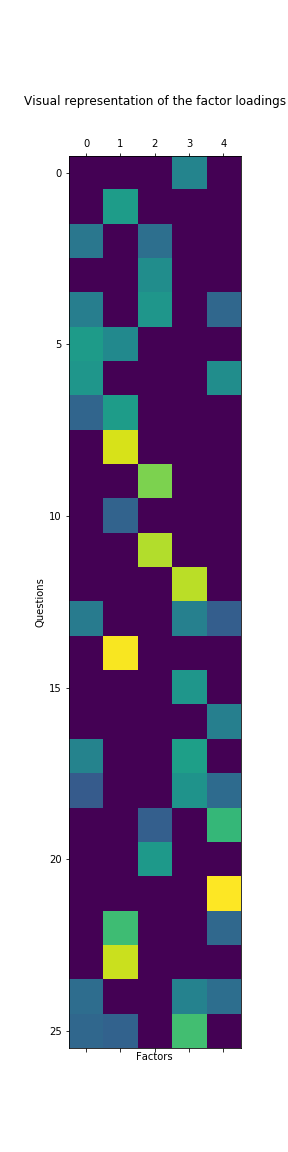
\includegraphics[scale=0.45]{factor_loadings.png}
  \caption{Visual representation of the factor loadings matrix with yellow being higher values that are approximately around 0.7 and lower values in green that are approximately around 0.3}
  %\rotatebox{90}
\end{figure}

\subsection{Convergent Validity Analysis}
For this part of the study, I decided to calculate the Cronbach alpha coefficient to test the internal validity of the data for all the scales \cite{cronbach}; you can refer to the values for each scale in table 2. As indicated by the internal validity for the scales, each scale does surprisingly well which is not a surprise as depicted by previous literature \cite{Leonard:2015}. In order to assess the internal validity the values for the state scale were divided into their respective subscales that were intended to measure the gambling fallacies stated above. With respect to the BIGLS scale, it was only used to measure convergence with respect to belief in luck \cite{darke:1997}. Additionally, the GRCS has three measures for illusion of control titled interpretive control/bias, illusion of control, and predictive control; similarly, the questions that measured illusion of control in the state scale were also separated and combined into a single matrix \cite{raylu:2004}. The other measures inside the GRCS are titled gambling related expectancies and perceived inability to stop gambling \cite{raylu:2004}. Since this study does not draw from a population of problematic gamblers, the perceived inability to stop gambling was excluded \cite{raylu:2004}. It should be noted that the only convergent analysis that could be conducted between the GRCS and BIGLS scale was only illusion of control and luck.

The first graph in figures 2 and 3 is the correlation coefficient value each subscale reports  with respect to the state scale. In other words, the correlation coefficient was calculated using the scores from the state scale and the scores from the GRCS or BIGLS. For each subscale, there was a 1-dimensional matrix that reported the scores for the state scale, GRCS, and the BIGLS. These matrices were used to calculate a correlation coefficient with the state scale against either the BIGLS or GRCS. These calculations were done through numpy's corrcoef function that uses a Pearson product-moment correlation coefficient. Since the BIGLS only measures luck, the correlation coefficient matrix was only calculated for the luck subscale and not for the illusion of control. Additionally, due to the nature of the 1-dimensional matrices, a correlation coefficient matrix only returns 1 unique value which is because the only thing being correlated is the score on each subscale.

The second graph in figures 2 and 3 indicate the overall score for each scale (i.e. GRCS, BIGLS, the state scale, and the pilot study state scale). Here the pilot study scores are relevant because the scores each participant gave can be compared to other participants of the state scale. Additionally, the subscales were plotted using a linear model that fit each participants reported score. Using numpy's polyfit function, the slope was calculated using each participant and their scores as (x,y) values. Put simply, each participant reported a score which was taken as the y value and the x-value was their participant number; for example, the first participant would have been number 1 and the last 101. 

The total score for each subscale was calculated via a sum of the number of scores participants reported for each sub-scale. Consideration was taken for having the number of subscales reflect a higher score on the graph simply because there is more subscales of one scale over another. In other words, if you have more subscales of, for example, the GRCS over the state scale then the GRCS sum would be more than the state scale. This was mitigated against by calculating an average before plotting the values; this means that the slope of the line is not important but rather the score they gave per each scale; it is more important to judge the relationship between each line rather than the score they gave which could be misleading otherwise.

\begin{figure}
  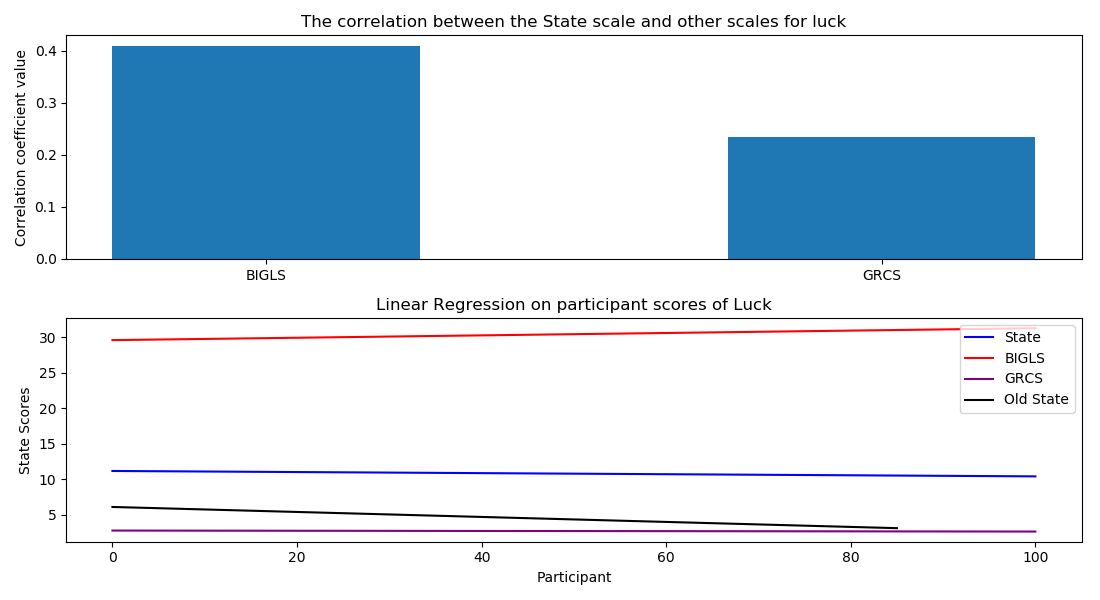
\includegraphics[scale=0.3, width=\columnwidth]{luck.png}
  \caption{Top figure: The relationship between the state scale and the other scales as reported by the correlation coefficient value via Numpy's corrcoef function for the luck subscale. Bottom figure: The total score each participant each on the luck subscale questions for the state scale, BIGLS, and the GRCS.}
  \centering
\end{figure}

\begin{figure}
  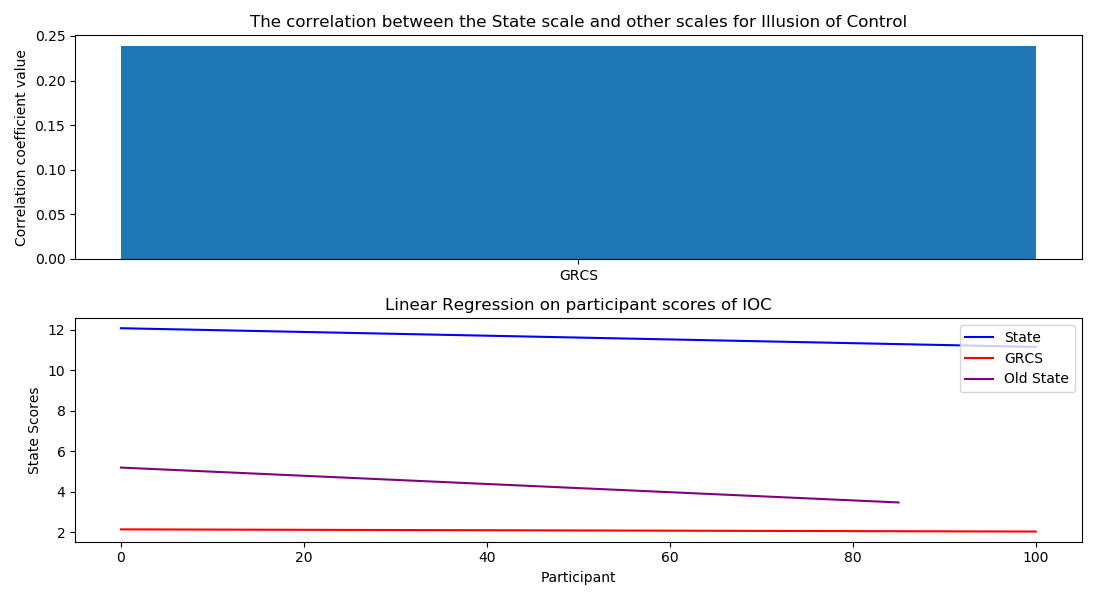
\includegraphics[scale=0.3, width=\columnwidth]{illusion_of_control.png}
  \caption{Top figure: The relationship between the state scale and the other scales as reported by the correlation coefficient value via Numpy's corrcoef function for the illusion of control subscale.. Bottom figure: The total score each participants of the illusion of control subscale}
  \centering
\end{figure}


\begin{table}
\caption{Cronbach's $\alpha$ for each study; a measure for internal validity of a scale used by the GRCS and BIGLS scale \cite{cronbach}}
\centering
\begin{tabular}{llr}
\toprule
\multicolumn{2}{c}{Cronbach's $\alpha$ coefficient} \\
\cmidrule(r){1-2}
Scale & Coefficient value \\
\midrule
State 2.0 & 0.922 \\
GRCS & 0.926\\
BIGLS & 0.904\\
Pilot & 0.899 \\
\bottomrule
\end{tabular}
\end{table}


%------------------------------------------------

\section{Results}

\subsection{Exploratory factor analysis (EFA)}
Since the EFA procedure was only used to drop the questions that were not identifying the latent factors clearly, the results of the questions dropped are not of particular value. However, it is important to address which questions were dropped and for what reason; since the removal of questions has a subjective nature such that some items that I might warrant removal, my supervisor would not. Due to this, the questions I removed were compared with those of my supervisor Gabriel Brooks. As a result, the factor loadings were clearly different and so were the eigenvalues that stated the explained variance. The questions I had dropped returned 5 latent factors as indicated by the five $\lambda$ values in figure 4 that are greater than 1; the five values include the $\lambda_0$ value. As noted previously, I lacked the experience of reducing questions in the pilot study so my choices for removing the questions were less liberal. This resulted in the five factors that were measuring belief in luck, illusion of control, supernatural belief, anthropomorphism, and the hot hand fallacy. In addition to the EFA question elimination procedure, I used the correlation coefficients to inform my decision such that those questions that reported a high correlation coefficient for each subscale were not removed \cite{efa}.

With each iteration of the question removal and procedure of checking the values, the Cronbach's $\alpha$ coefficient was calculated as listed in table 1. This indicates that the results of the convergent validity analysis would  be meaningful because the questions in each scale were high in internal validity \cite{cronbach}. Additionally, the value reported by the "State 2.0" scale in table 1 were higher than that of the pilot study. These values were calculated after the questions were removed from both the state scale and the pilot study scale. Moreover, the higher values for the state scale suggest that the removal of the questions were more effective than the pilot study and that each question was measuring its intended variable \cite{cronbach}. Put simply, the questions in the state scale were performing consistently and that the change in questions from the pilot study scale was effective.

\begin{figure}
  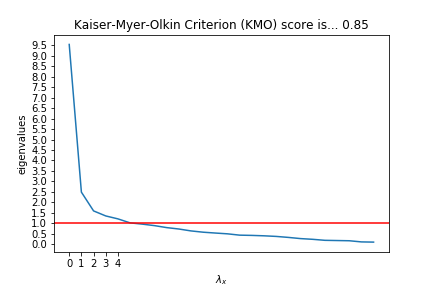
\includegraphics[scale=0.3, width=\columnwidth]{scree_test.png}
  \caption{The plot of eigenvalues according to the state scale scores with the KMO value reported. Note that a value of 0.85 indicates that the state scale sample size was suitable for EFA \cite{efa}. The x-axis is the $\lambda$ value which indicates individual latent factors. The y-axis indicates the variance accounted for by each eigenvalue \cite{efa}}
  \centering
\end{figure}


Additionally, the results of the questions dropped by my supervisor resulted in 4 latent factors that measured gambling fallacies such as anthropomorphism, the gamblers fallacy, the hot hand fallacy, and  illusion of control. This is interesting because the questions removed were more liberal than my own and as a result, the factor loadings were clearly defined for each question. Moreover, the KMO value was also high indicating that even after removing a list of questions, the suitability of the data to the sample size had not changed significantly. It should also be noted that my supervisor used a different rotation method than mine but both methods assume that the factors are related to each other rather than being orthogonal; the method I used was the "quartimin" rotation and the one my supervisor used was the "oblimin" \cite{efa}. 

\subsection{Convergent Validity Analysis}
As shown by figure 2, the correlation values in the luck subscale indicate a moderate correlation with the BIGLS \cite{correlation}. As was expected however, the correlation between the GRCS and the state scale for the luck subscale was low; it is also apparent with the second figure because it gives a better depiction of how poorly the GRCS evaluates luck. In the second plot, the GRCS' values are extremely lower than that of the BIGLS, state scale, and pilot study scale. However, the BIGLS performs very highly on scores of luck as reported by the second plot. In addition to the high internal reliability reported by the Cronbach's alpha coefficient, it suggests that the BIGLS scale is accurately predicting the values retained with respect to luck. Additionally, since the state scale also reports higher values in the second plot and the correlation coefficient returns a moderate relationship, it suggests that the state scale is measuring luck fairly well. The discrepancy between the gap in the lines depicted in the second plot should be interpreted using the correlation coefficient values. This is because the score a participant gives on luck does not, at first glance, tell you how well the question is performing so the correlation coefficient must be considered.

Also, figure 3 depicts the relationship of the state scale with respect to the GRCS for illusion of control. It is interesting that the correlation coefficient for the illusion of control (IOC) is low but it is somewhat expected. This is because the subscales inside the GRCS measuring IOC includes different phrasing and tries to capture "interpretive control/bias", "illusion of control", and "predictive control" \cite{raylu:2004}. These questions are different such that the state scale measures not only IOC but also anthropomorphism which exerts a normative social influence \cite{wyatz:2010}. The differences between the two scales could also explain the second plot in which the state scale and the pilot study scale report higher scores than the GRCS itself. An explanation of this could be that as a result of the gambling experience and the "double switching" concept, the higher scores reflect not only a different measure but a result of the gambling itself since the GRCS scores were taken prior to the gameplay \cite{sevigny:2003}. The lower correlation coefficient also reflects the difference of scores in the second plot but that could be a result of the fact that the state scale measures different aspects of IOC. Additionally, the scores of the pilot study data are also reflected in the second plot and lends to the idea that even though the gambling experience might have played a role, it was the question that ultimately decided the scores. This is because the GRCS scores in the second plot is closer to the pilot study data than the state scale. This suggests that the phrasing of the IOC questions produced the higher values in spite of the gambling experience. The gambling experience could possibly account for the higher scores from the pilot study data than the GRCS. 
%------------------------------------------------


\section{Discussion}
The goal of this study was to decide if a session of slot machine gameplay could affect the reported score of a gambling related cognitions scale such that values of a subscale in a reliable measure (i.e. GRCS or BIGLS) reflects a strong relationship to the state scale. The results indicate that this is possibly the case since the correlation coefficient that was reported in the luck subscale reflects a moderate relationship \cite{correlation, darke:1997}. In addition to its high internal reliability, the BIGLS and the state scale scores provide evidence to suggest that the relationship between the two is a meaningful one \cite{cronbach, efa, correlation}. With respect to the GRCS scale, the low correlation coefficient and the difference in scores could possibly be a result of the way the GRCS measures illusion of control \cite{raylu:2004}. However, this is mitigated against by the EFA where the factor loadings load onto one measure more strongly than others \cite{efa}. It should also be noted that the GRCS scale did not include a gambling component whereas the "double switching" concept would suggest that such an experience plays a significant role in determining the persons beliefs \cite{raylu:2004, sevigny:2003}.

Additionally, it is important to mention that this article reviews a part of the larger academic endeavour for this research such that another group of participants will be examined afterwards. These group of participants are needed so that the changes in their reported score is accounted for by their gambling experience; as with the participants in this group they will play a slot machine session but watch the videos of gameplay before doing so. It is suggested that after watching another person play a slot machine, the beliefs one might hold could be reflected in the scores on the state scale. Moreover, the second group of participants will show that the results of the EFA are due to the changes in gambling experience; this is not accounted for by the GRCS so a possible explanation of the low scores in illusion of control can be explained through this manipulation \cite{raylu:2004}.

The possibly implications for such research indicates that measuring the facets of gambling related cognitions will be more thorough; the thoroughness refers to the fact that existing scales do not measure the breadth of gambling fallacies but rather focus on a subset \cite{Leonard:2015}. Additionally, it could aid in clinical diagnosis of pathological gambling such that it could provide clarification on the particular erroneous beliefs a person is more susceptible to that might have lead to a pathological gambling issue \cite{xian:2008, Ladouceur:2004}. Lastly, this will hopefully provide more evidence towards the research of gambling related cognitions.

%----------------------------------------------------------------------------------------
%	REFERENCE LIST
%----------------------------------------------------------------------------------------

\begin{thebibliography}{99} % Bibliography - this is intentionally simple in this template

%\bibitem{Figueredo:2009dg}
%Figueredo, A.~J. and Wolf, P. S.~A. (2009).
%\newblock Assortative pairing and life history strategy - a cross-cultural
%  study.
%\newblock {\em Human Nature}, 20:317--330.
\bibitem[Leonard et al., 2015]{Leonard:2015}
  Leonard, Carrie A., Robert J. Williams, and John Vokey. "Gambling fallacies: what are they and how are they best measured?." (2015).

\bibitem[Ladouceur, 2004]{Ladouceur:2004}
  Ladouceur, R. (2004). Perceptions among pathological and nonpathological gamblers. \emph{Addictive behaviors, 29}(3), 555-565.

\bibitem[Raylu and Oei, 2004]{raylu:2004}
  Raylu, N., \& Oei, T.P. (2004). The Gambling Related Cognitions Scale (GRCS): Development, confirmatory factor validation and psychometric properties. \emph{Addiction, 99}(6), 757-769.

\bibitem[Se'vigny \& Ladouceur, 2003]{sevigny:2003}
  Se'vigny, S., \& Ladouceur, R. (2003). Gamblers' irrational thinking about chance events. The 'double switching' concept. \emph{International Gambling Studies, 3}(2), 149-161.

\bibitem[Xian et. al., 2008]{xian:2008}
  Xian, H., Shah, K.R., Phillips, S.M., Scherrer, J.F., Volberg, R., \& Elsen, S.A. (2008). Association of cognitive distortions with problem and pathological gambling in adult male twins. \emph{Psychiatry research, 160}(3), 300-307.

\bibitem[Wyatz et. al., 2010]{wyatz:2010}
  Wyatz, A., Cacioppo, J., \& Epley, N. (2010). Who sees human? The stability and importance of individual differences in anthropomorphism. \emph{Perspectives on Psychological Science, 5}(3), 219-232.

\bibitem[Fabrigar and Duane, 2012]{efa}
  Fabrigar, L.R., \& Wegener, D.T. (2012). \emph{Exploratory Factor Analysis}. New York,NY: Oxford University Press, Inc.

\bibitem[Darke and Freedman, 1997]{darke:1997}
  Darke, P.R., \& Freedman, J.L. (1997). The belief in good luck scale. \emph{Journal of research in personality, 31}(4), 486-511.

\bibitem[Gabriel B., personal communication, March 2019]{gabriel}
  Gabriel, B. (2019, March). Personal communication.

\bibitem[Santos, 1999]{cronbach}
  Santos, J.R.A. (1999). Cronbach's alpha: A tool for assessing the reliability of scales. \emph{Journal of extension, 27}(2), 1-5.

\bibitem[Ejova et. al., 2015]{ejova:2015}
  Ejova, A., Delfabbro, P.H., \& Navarro, D.J. (2015). Erroneous gambling-related beliefs as illusions of primary and secondary control: A confirmatory factor analysis. \emph{Journal of Gambling Studies, 31}(1), 133-160.

\bibitem[Biggs, 2017]{factoranalyzer}
  Biggs, J. (2017). FactorAnalyzer. Retrieved from https://factor-analyzer.readthedocs.io/en/latest/

\bibitem[Wynne, 2003]{wynne:2003}
  Wynne, H. (2003). Introducing the Canadian problem gambling index. \emph{Edmonton, AB: Wynne Resources.}

\bibitem[Lay, 2012]{lay}
  Lay, David C. \emph{Linear Algebra and Its Applications.} Addison-Wesley, 2012.

\bibitem[Rush et. al., 2008]{rush:2008}
  Rush, B.R., Bassani, D.G., Urbanoski, K.A., \& Castel, S. (2008). Influence of co-occurring mental and substance use disorders on the prevalence of problem gambling in Canada. \emph{Addiction, 103}(11), 1847-1856.

\bibitem[BCLC, 2018]{bclc}
  British Columbia Lottery Corporation. (2018). \emph{Responsible Gambling in British Columbia}[Fact sheet]. Retrieved from https://corporate.bclc.com/content/dam/bclc/corporate/documents/fact-sheets/fs-responsible-gambling-bc.pdf

\bibitem[Pearson's Correlation using Stata. (n.d.)]{correlation}
  Pearson's Correlation using Stata. (n.d.) Retreived from https://statistics.laerd.com/stata-tutorials/pearsons-correlation-using-stata.php

\end{thebibliography}

%----------------------------------------------------------------------------------------

\end{document}
